\paragraph{Control Chemotherapy for HIV} 
	Now we discuss a optimal control mode to describe the effect of chemotherapy
in the interaction between the HIV virus and $CD4^+T$ cells 
\cite{butler1997optimal}.


The optimal control problem reads:
\begin{equation}
	\begin{aligned}
		\max_{u} & \int_{0}^{t_{final}}
			A  T(t) - (1-u(t)) ^ 2 dt
		\\
		\text{s.t. }
		\\
			T'(t) &=
				\frac{s}{1 + V(t)}
				- m_1 T(t) 
				+ r T(t)
				\left[
					1 - \frac{T(t)+ T_{I}(t)}{T_{max}}
				\right] 
				- u(t) k V(t) T(t),
			\\
			T_{I}(t) &=
				u(t) k V(t) T(t) - m_2 T_{I}(t),
			\\
			V'(t) &= N m_2 T_{I}(t) - m_3 V(t),
			\\
	\end{aligned}
\end{equation}

\begin{figure}[tbh]
\centering
	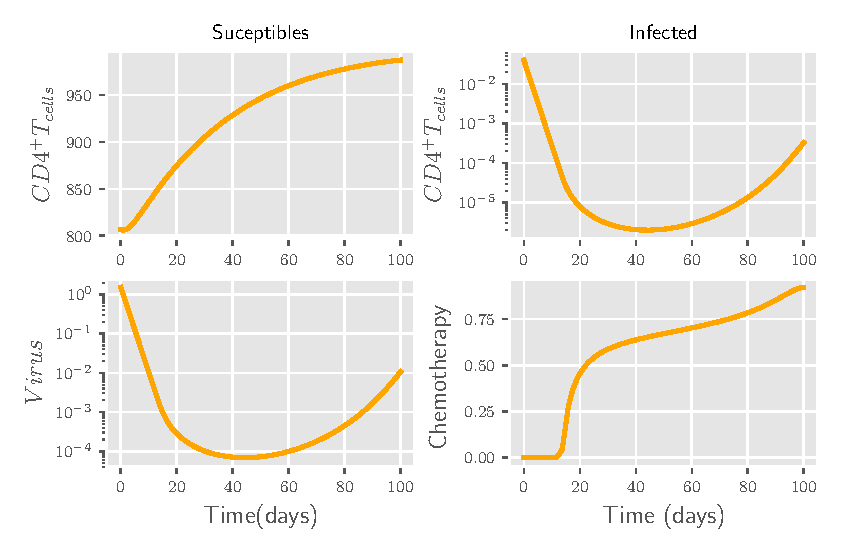
\includegraphics[width=0.7\linewidth]{Figures/hiv_chemotherapy_fig_01}
	\caption{Add description and stress the schedule of treatment}
	\label{fig:hivchemotherapyfig01}
\end{figure}
